\documentclass[10pt]{article}
\usepackage{icmlko}

\icmlmeta{IP 파운데이션 월드모델}{197}{풀링은 닮아서가 아니라 업어 주기 때문이다}{노트 196이 남긴 제일 큰 줄 --- ``풀링은 열 도메인의 라벨이 같은 것을 묻는다고 가정한다.'' 정면으로 쟀더니 가정은 넷에서 거짓인데 풀링은 여전히 이긴다. 까닭이 다른 데 있었다}

\begin{document}

\twocolumn[
\icmlheader

\begin{abstract}
이 실험실의 얼개는 열 도메인의 계수를 나눠 쓰는 풀링이고(노트 5), 노트
181이 ``애니 라벨은 속편을 벌하고 세계애니 라벨은 안 벌한다''를 재면서
그 가정에 처음 금을 냈다. 정면으로 쟀다. \textbf{① 계수는 서로 반대를
가리키지 않는다} --- 도메인마다 따로 능형을 적합해 계수 벡터를 뽑으면
쌍 코사인 스물하나가 \textbf{전부 양수}이고 중앙이 $+$0.455 다(범위
$+$0.03$\sim$$+$0.81). \textbf{다만 도서는 다르다} --- 판 계수와 코사인이
0.208 인데, 학습 표본이 80건뿐이라 잡음일 수 있어 통제했다. 다른 도메인을
전부 80건으로 깎아도 코사인이 0.37$\sim$0.58 로 남는다 --- \textbf{도서의
낮음은 표본 탓이 아니다.} \textbf{② 넷은 따로 하는 것이 낫다.} 완전 분리
$+$0.3445 대 완전 풀링 $+$0.3822 로 풀링이 이기는데, 갈라 보면 일곱 중
\textbf{넷}(모바일 $+$0.076 · 세계애니 $+$0.022 · 펀딩 $+$0.035 · 도서
$+$0.013)이 혼자가 낫고 둘(웹툰 $+$0.158 · 게임 $+$0.108)만 크게 얻는다.
\textbf{③ 무엇이 그 이득을 정하나.} 후보 넷을 견줬다 --- 학습 표본
($\rho{=}-0.07$) · 판 계수와의 코사인($-0.25$) · 유보 표본($+0.43$) ·
\textbf{혼자 학습했을 때의 $\rho$($\mathbf{-0.54}$ · 피어슨 $-0.60$)}.
\textbf{풀링은 자기 자료로 못 배우는 도메인을 업어 주는 장치다} --- 웹툰은
혼자 $+$0.090 이라 $+$0.158 을 얻고 모바일은 혼자 $+$0.514 라 $-$0.076 을
잃는다. \textbf{닮아서가 아니다.} ④ 그러면 도메인마다 골라 주면 된다.
안쪽 시간 분할로 ``혼자 대 풀링''을 견주어 고르니 판이 $+$0.3822 에서
\textbf{$+$0.3965} 가 된다. 문턱을 걸어 갈라 보니 \textbf{0.02$\sim$0.10
어디서든 $+$0.3955} 로 같고, 그중 \textbf{모바일 하나가 $+$0.0133 으로
93\%}다. 노트 178 · 182 의 문턱이 한 칸 옆에서 뒤집히던 것과 대조된다.
\end{abstract}
]

\begin{figure*}[t]
\centering
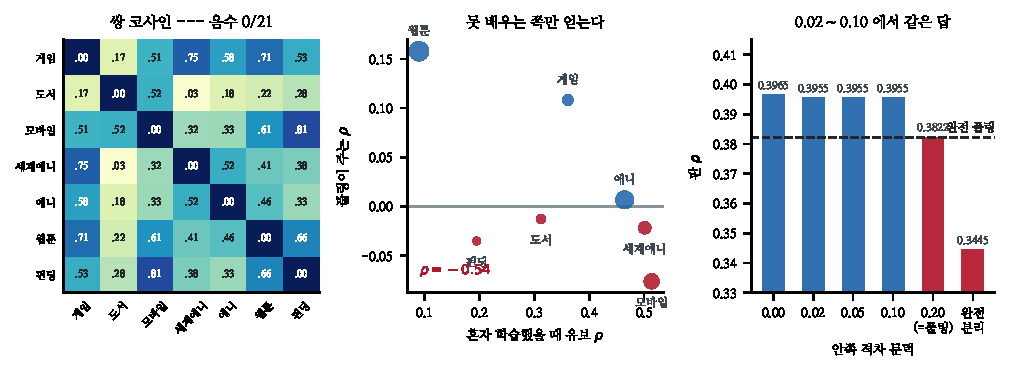
\includegraphics[width=\textwidth]{figs/carry.pdf}
\caption{왼쪽 --- 쌍 코사인은 음수가 없다. 가운데 --- 못 배우는 쪽만 얻는다.
오른쪽 --- 문턱 0.02$\sim$0.10 에서 같은 답.}
\end{figure*}

\section{계수는 반대를 안 가리킨다}

\begin{table}[t]
\centering\tsize
\caption{도메인마다 따로 적합한 계수. 공통 축 열아홉 $\times$ 2(값·표시자).}
\begin{tabular}{lrr}
\toprule
& 학습 n & 판 계수와 코사인 \\
\midrule
세계애니 & 2{,}648 & .729 \\
게임 & 259 & .674 \\
모바일 & 1{,}559 & .609 \\
펀딩 & 320 & .537 \\
웹툰 & 2{,}106 & .528 \\
애니 & 1{,}467 & .503 \\
\textbf{도서} & \textbf{80} & \textbf{.208} \\
\midrule
\multicolumn{2}{l}{쌍 코사인 중앙} & $+$.455 \\
\multicolumn{2}{l}{음수인 쌍} & \textbf{0 / 21} \\
\bottomrule
\end{tabular}
\end{table}

\claimx{\textbf{스물한 쌍이 전부 양수다.} 라벨이 서로 \emph{반대}를 묻지는
않는다 --- 노트 180이 위키 축 하나에서 본 부호 뒤집힘이 계수 전체로는
안 나타난다.}{다만 중앙 $+$0.455 는 ``닮았다''고 하기엔 낮다. 같은 질문을
묻는다면 0.8 을 넘어야 한다.}

\claimx{\textbf{도서만 다르고, 표본 탓이 아니다.} 다른 도메인을 전부 80건으로
깎아도 코사인이 0.37$\sim$0.58 인데 도서는 0.21 이다.}{도서 축은 알라딘
메타(쪽수 · 판형 · 무게 · 정가)라 다른 도메인과 재는 것이 제일 다르다
(\texttt{docs/AXIS\_MEANING.md}). \textbf{표본을 통제하니 그것이 드러난다.}}

\section{넷은 따로가 낫다}

\begin{table}[t]
\centering\tsize
\caption{같은 알파(20)로 셋을 견준다.}
\begin{tabular}{lrrrr}
\toprule
& n & 완전 분리 & 풀링$+$절편 & 차 \\
\midrule
\textbf{웹툰} & 711 & \textbf{.0902} & \textbf{.2478} & \textbf{$+$.158} \\
\textbf{게임} & 223 & .3612 & \textbf{.4693} & \textbf{$+$.108} \\
애니 & 606 & .4644 & .4710 & $+$.007 \\
도서 & 163 & .3125 & .2998 & $-$.013 \\
세계애니 & 300 & \textbf{.5011} & .4793 & $-$.022 \\
펀딩 & 80 & \textbf{.1954} & .1602 & $-$.035 \\
\textbf{모바일} & 441 & \textbf{.5137} & .4375 & \textbf{$-$.076} \\
\midrule
\textbf{판} & 2{,}524 & \textbf{.3445} & \textbf{.3822} & \\
\bottomrule
\end{tabular}
\end{table}

\claimx{\textbf{판은 풀링이 이기는데 도메인은 넷이 진다.} 이기는 둘이 크고
약해서 판을 끌어올린다 --- 웹툰이 유보 711건으로 판의 28\%다.}{\textbf{노트
183이 잰 그 성질이다} --- 판은 크기 가중이라 작은 도메인의 손해를 숨긴다.
여기서는 큰 도메인의 이득이 작은 도메인들의 손해를 덮는다.}

\section{못 배우는 쪽만 얻는다}

\begin{table}[t]
\centering\tsize
\caption{풀링 이득을 무엇이 예측하나.}
\begin{tabular}{lrr}
\toprule
& 스피어만 & 피어슨 \\
\midrule
\textbf{혼자 학습한 $\rho$} & \textbf{$-$.536} & \textbf{$-$.602} \\
유보 표본 & $+$.429 & $+$.421 \\
판 계수와 코사인 & $-$.250 & $+$.084 \\
학습 표본 & $-$.071 & $+$.057 \\
\bottomrule
\end{tabular}
\end{table}

\claimx{\textbf{혼자 학습한 $\rho$ 하나가 예측한다.} 웹툰은 혼자 $+$0.090
이라 $+$0.158 을 얻고 모바일은 혼자 $+$0.514 라 $-$0.076 을
잃는다.}{\textbf{코사인은 거의 예측 못 한다}($-$0.25 · 피어슨 $+$0.08) ---
계수가 얼마나 닮았는지는 풀링의 값어치와 상관이 없다. \textbf{닮아서가
아니다.}}

\claimx{\textbf{그러니 풀링은 라벨 동질성의 증거가 아니다.} 자기 자료로
못 배우는 도메인을 업어 주는 장치이고, 잘 배우는 도메인에는 짐이다.}{노트
196이 남긴 질문에 답이 됐다 --- \textbf{가정은 넷에서 거짓인데 얼개는
여전히 이긴다.} 두 사실이 모순이 아니다.}

\section{도메인마다 골라 준다}

\begin{table}[t]
\centering\tsize
\caption{안쪽 시간 분할로 ``혼자 대 풀링''을 고른다. 유보 미접촉.}
\begin{tabular}{lrr}
\toprule
안쪽 격차 문턱 & 혼자 고른 도메인 & 판 \\
\midrule
0.00 & 모바일·세계애니·애니 & \textbf{.3965} \\
\textbf{0.02} & \textbf{모바일} & \textbf{.3955} \\
0.05 & 모바일 & .3955 \\
0.10 & 모바일 & .3955 \\
0.20 & (없음) & .3822 \\
\midrule
\multicolumn{2}{l}{완전 분리} & .3445 \\
\bottomrule
\end{tabular}
\end{table}

\claimx{\textbf{0.02$\sim$0.10 어디서든 같은 답이다}($+$0.3955). 노트 178 ·
182 에서 문턱이 한 칸 옆에서 부호를 뒤집던 것과 대조된다 --- \textbf{이번엔
답이 평평하다.}}{모바일의 안쪽 격차가 0.122 로 혼자 뚜렷하고 나머지는
0.003$\sim$0.021 로 잡음 수준이다. \textbf{한 도메인만 확실하니 문턱이
안 흔들린다.}}

\claimx{\textbf{모바일 하나가 이득의 93\%다}($+$0.0133 / $+$0.0143). 모바일은
유보 441건에 혼자 $\rho$ 가 $+$0.514 로 제일 잘 배우는 도메인이다 ---
\textbf{제일 잘 배우는 도메인을 풀에서 빼는 것이 제일 큰 이득이다.}}{채택은
문턱 0.02 쪽이 맞다 --- 0.00 이 $+$0.0010 더 높지만 그 셋 중 둘의 안쪽
격차가 0.003 · 0.014 로 잡음이다.}

\begin{table}[t]
\centering\tsize
\caption{남은 것.}
\begin{tabular}{ll}
\toprule
\textbf{중간} & 혼자/풀링 둘이 아니라 섞는 비율로 \\
도서 & 코사인 0.21 --- 축이 다른 것을 재고 있다 \\
트리 & 이 실험은 능형만 --- F18 은 안 쟀다 \\
\bottomrule
\end{tabular}
\end{table}

첫 줄이 곧바로 다음이다. 지금은 도메인마다 ``혼자냐 풀링이냐''를 이분으로
고르는데, 진짜 답은 그 사이에 있을 것이다 --- 노트 155의 F10 도메인별
축소가 바로 그 얼개인데 축소량을 하나로 쓴다. \textbf{도메인마다 축소량을
안쪽에서 고르면} 모바일은 거의 혼자, 웹툰은 거의 풀링으로 갈 것이고
$+$0.3955 를 넘을 수 있다. 그리고 그 축소량이 바로 이 노트가 잰 ``혼자
학습한 $\rho$''의 함수여야 한다 --- \textbf{예측자를 이미 찾았으므로 고르는
대신 계산할 수도 있다.}

\end{document}
